\documentclass[10pt]{article}
\usepackage{indentfirst}
\usepackage{hyperref}
\usepackage[dvips]{graphicx}
\usepackage{pst-plot}
\usepackage{mathrsfs}
\usepackage{epic,eepic}
\usepackage{amsfonts}
\usepackage{amsmath,amssymb}
\usepackage{bm}
\usepackage{enumitem}
\usepackage{subcaption}
\usepackage{braket}
% set up paper size
\setlength{\textwidth}{17.59cm}
\setlength{\marginparsep}{0pt}
\setlength{\marginparwidth}{0pt}
\setlength{\textheight}{24.05cm}
\setlength{\headheight}{0pt}
\setlength{\headsep}{0pt}
\setlength{\oddsidemargin}{-0.04cm}
\setlength{\topmargin}{-.04cm}

\renewcommand{\baselinestretch}{1.1}


\begin{document}

\thispagestyle{empty}
     \rule{\linewidth}{1mm}
     \begin{flushright}
           \Huge From Quarks to Stars: A Quantum Computing Approach to the Nuclear Many-Body Problem
     \end{flushright}
     \rule{\linewidth}{1mm}
     \vspace*{\stretch{2}}
 \begin{center}
 \begin{figure}[hb]
 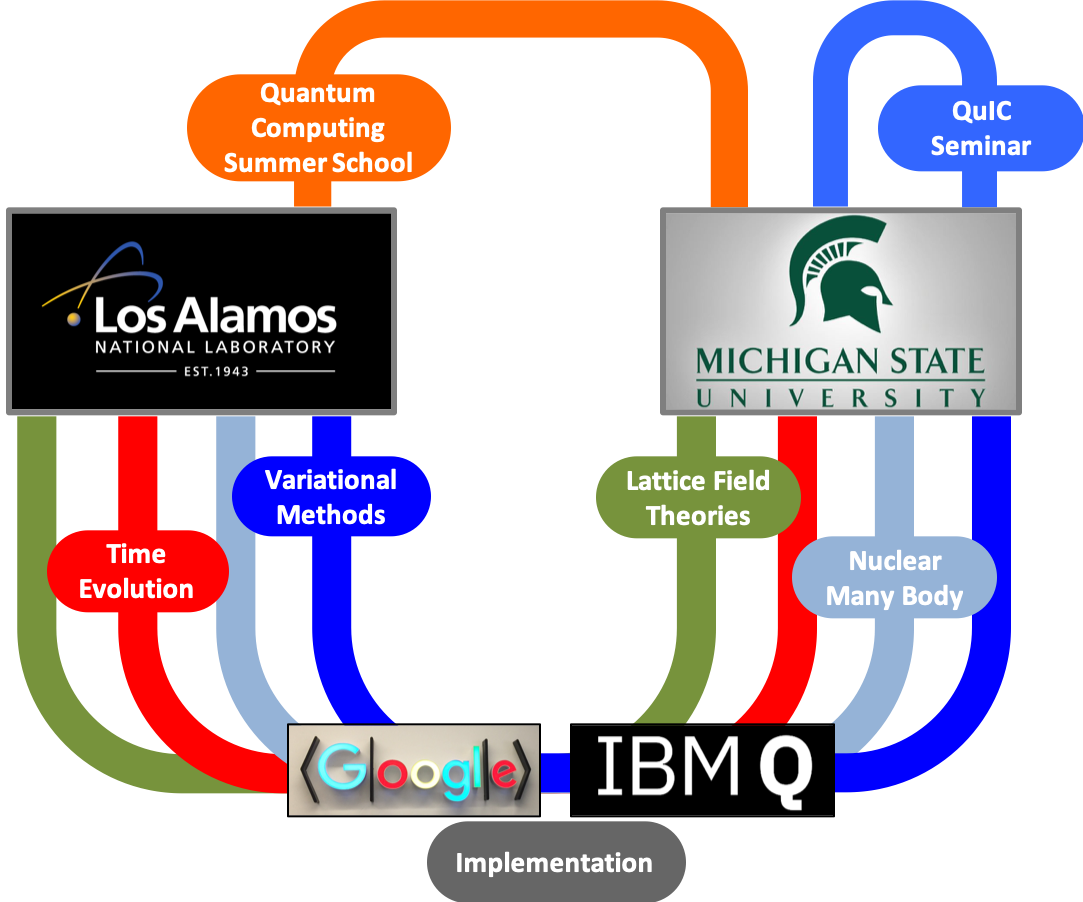
\includegraphics[scale=1.0]{Figures/NP_Collaboration.png}
 \end{figure}
 \end{center}
\newpage
\title{DOE Quantum Horizons: QIS Research and Innovation for Nuclear Science}
\maketitle
\rule{\linewidth}{1mm}
\begin{flushleft}
{\bf Title: From Quarks to Stars: A Quantum Computing Approach to the Nuclear Many-Body Problem}\newline
Institution: Facility for Rare Isotope Beams and Michigan State University\newline
Address: 640 S.~Shaw Lane, East Lansing, MI 48824\newline
Administrative point of Contact: Chris West, westc@frib.msu.edu (add phone) \newline
Lead Principal Investigator: Morten Hjorth-Jensen\newline
DOE Funding Opportunity Announcement (FOA) Number: DE-FOA-0002110\newline
FOA type: Initial\newline
CDFA Number: 81.049\newline
DOE/Office of Science Program Office: {\bf Nuclear Physics}\newline
DOE/Office of Science Program Office Technical Contact: Dr. Gulshan Rai (301-903-4702), gulshan.rai@science.doe.gov\newline
Research Area: Theoretical Nuclear Physics; Computational Many-body Physics; Lattice Quantum Chromodynamics; Quantum Algorithms; Quantum Simulations
\end{flushleft}
\rule{\linewidth}{1mm}
\begin{table}[hbtp]
\caption{List of Team Members}
\begin{center}
\begin{tabular}{|l|l|l|l|}
\hline
\multicolumn{3}{|l}{{\bf Team Members} } & \multicolumn{1}{|l|}{{\bf Institution}}\\
\hline
\multicolumn{1}{|l}{Last Name} & \multicolumn{1}{|c|}{First Name} & \multicolumn{1}{l|}{Title} & \multicolumn{1}{l|}{Institution Name} \\
\hline
Bazavov & Alexei & Assistant Professor & Michigan State University \\
\hline
Bogner & Scott & Professor & Michigan State University \\
\hline
Hergert & Heiko & Assistant Professor & Michigan State University \\
\hline
Hirn & Matthew & Assistant Professor & Michigan State University \\
\hline
Hjorth-Jensen & Morten & Professor & Michigan State University, University of Oslo\\
\hline
Lee & Dean & Professor & Michigan State University \\
\hline
Lin & Huey-Wen & Assistant Professor & Michigan State University \\
\hline
Shindler & Andrea & Associate Professor & Michigan State University \\
\hline
Coles & Patrick & Senior Scientist & Los Alamos National Laboratory \\
\hline

\end{tabular}
\end{center}
\end{table}

\newpage
\tableofcontents
\section{Executive Summary}

Michigan State University (MSU) and the Facility for Rare Ion Beams (FRIB) are submitting 
a proposal on {\bf From Quarks to Stars: A Quantum Computing Approach to the Nuclear Many-Body Problem}. 

{\bf Intellectual merit:} For nuclear theorists, the overarching
challenge is to develop a comprehensive description of nuclei and
their reactions, grounded in the fundamental interactions between the
constituent nucleons with quantifiable uncertainties to maximize
predictive power.  As experimental frontiers have shifted to the study
of rare isotopes, the predictive power of successful phenomenological
approaches like the shell model and density functional theory is
challenged by the scarcity of nearby experimental data to constrain
model parameters. Therefore, it is expected that \emph{ab initio}
methods will play an increasingly prominent role to help improve the
predictive power of such ``data driven'' methods as experiment moves
deeper into largely unexplored regions of the nuclear chart.

To understand why nuclear matter is stable, and thereby shed light on
the limits of nuclear stability, is one of the overarching aims and
intellectual challenges of basic research in nuclear physics. To
relate the stability of matter to the underlying fundamental forces
and particles of nature as manifested in nuclear matter, is central to
present and planned rare isotope facilities such as the DOE facility
FRIB under construction at Michigan State University.  From a
theoretical standpoint, this involves understanding how the basic
building blocks of Nature interact and conspire to build up atomic
nuclei as we know them, with the aim to understand what makes visible
matter stable.  The theoretical efforts span from methods like Lattice
Quantum Chromodynamics, via effective field theories to many-body
theories applied to atomic nuclei and infinite nuclear matter. All
these methods rely on theoretical approximations whose applicabilities
are often limited by the dimensionality of the specific problem being
studied. In recent years there has been considerable progress in our
theoretical understanding of algorithms from quantum information
applied to interacting systems, with the hope to circumvent many of
the traditional dimensionality problems.


This proposals unites the efforts of nuclear many-body theorists,
quantum information theorists and mathematicians, with the aim to
explore and develop stable algorithms for studying nuclear systems
using recent progress in quantum information theory. It involves
researchers from Michigan State University (MSU) and the National
Superconducting Cyclotron Laboratory (NSCL)/Facility for Rare Ion
Beams (FRIB) and Los Alamos National Laboratory, with the aim to build
up an interdisciplinary team of nuclear theorists and quantum
information theorists in order to explore the feasibility of quantum
information theory applied to the nuclear many-body problem.


{\bf Broader impacts:} The training received by undergraduates,
graduate students, and postdoctoral research associates in carrying
out the proposed activities contributes directly to the building of a
diverse scientific workforce. The present proposal has a large
educational component, being part of the nuclear physics program at
FRIB/MSU that was recently ranked number one in the country. The mix
of analytical and numerical computations our students must employ is
an excellent preparation for both academic and industrial research. The
PIs are committed to diversity in science.


\section{Introduction and Scientific Motivation}

\subsection{The overarching intellectual question(s)}

Can we understand nuclei and nuclear matter and the limits of
stability of matter in terms of the fundamental laws of motion and
forces?  Stated differently, can we relate  what we observe experimentally
to the properties of the strong force and its underlying theory
Quantum Chromodynamics?

One of the fundamental intellectual challenges in nuclear physics is to understand
why nucleonic matter is stable, how it comes into being, how it
evolves and organizes itself, and what phenomena emerge. The task
facing nuclear theorists is to develop the tools to help answer these
questions by relating the existence and properties of nuclei to the
underlying fundamental forces and degrees of freedom. As experimental
efforts have shifted towards the study of rare
isotopes, there
has been an increased urgency to develop reliable 
calculations to counter the inherent limitations of ``data-driven''
approaches which rely on experimental data to constrain model
parameters, such as the phenomenological shell model and density
functional theory. 

For decades progress in nuclear few- and many-body theory was slowed
by the lack of a consistent theory for the strong inter-nucleon
interactions, and by the computational demands required to handle the
non-perturbative aspects resulting from the ``hard cores'' and strong
tensor forces found in most interaction models.  For many years, the
only option for controlled calculations was to use quasi-exact methods
such as quantum Monte Carlo (QMC) or no-core shell model (NCSM), which
limited the reach of so-called \emph{ab initio}\footnote{The concept
  \emph{ab initio} or first principle calculations is normally
  reserved to calculations performed in terms of the underlying forces
  and elementary particles. In several few- and many-body communities
  this has been extended to mean exact or quasi-exact calculations
  with a given input Hamiltonian/Lagrangian. The latter is not
  necessarily the one which relates directly to the fundamental
  bulding blocks.} calculations to light $p$-shell nuclei. Approximate
(but systematically improvable) methods that scale favorably to larger
systems, like coupled cluster (CC) theory and many-body perturbation
theory (MBPT), were largely abandoned in nuclear physics, despite
enjoying tremendous success in quantum chemistry.


Much has changed in recent years, as advances in chiral effective
field theory (EFT), which provides a systematic framework to construct
consistent two- and three-nucleon
interactions,
together with the development of powerful many-body methods have
pushed the
frontiers of \emph{ab initio} theory well into the medium-mass
region, see Fig.~\ref{fig:abinitio}. 
Initial applications of these methods were limited primarily to ground-state
properties of stable nuclei near shell closures with two-nucleon
forces only. Substantial progress has since been made on including
three-nucleon forces, targeting excited states and observables besides
energy, and moving into the more
challenging terrain of open-shell and unstable
nuclei. % add references
The recent work of Jansen {\em et al} \cite{jansenprl2016} on the structure of $^{78}$Ni and nearby nuclei represents some of the progress which has been made recently in pushing the limits of first principle methods. Remarkably,
progress on the many-body front has been so swift in recent years that
inadequacies of the current-generation chiral two- and three-nucleon
interactions, rather than the many-body calculations themselves, are
the primary obstacles to systematic calculations across the
medium-mass region~\cite{Ekstrom2015}.

\begin{figure}[t!]
\centering
   \begin{subfigure}[t]{.5\textwidth}
   \centering
  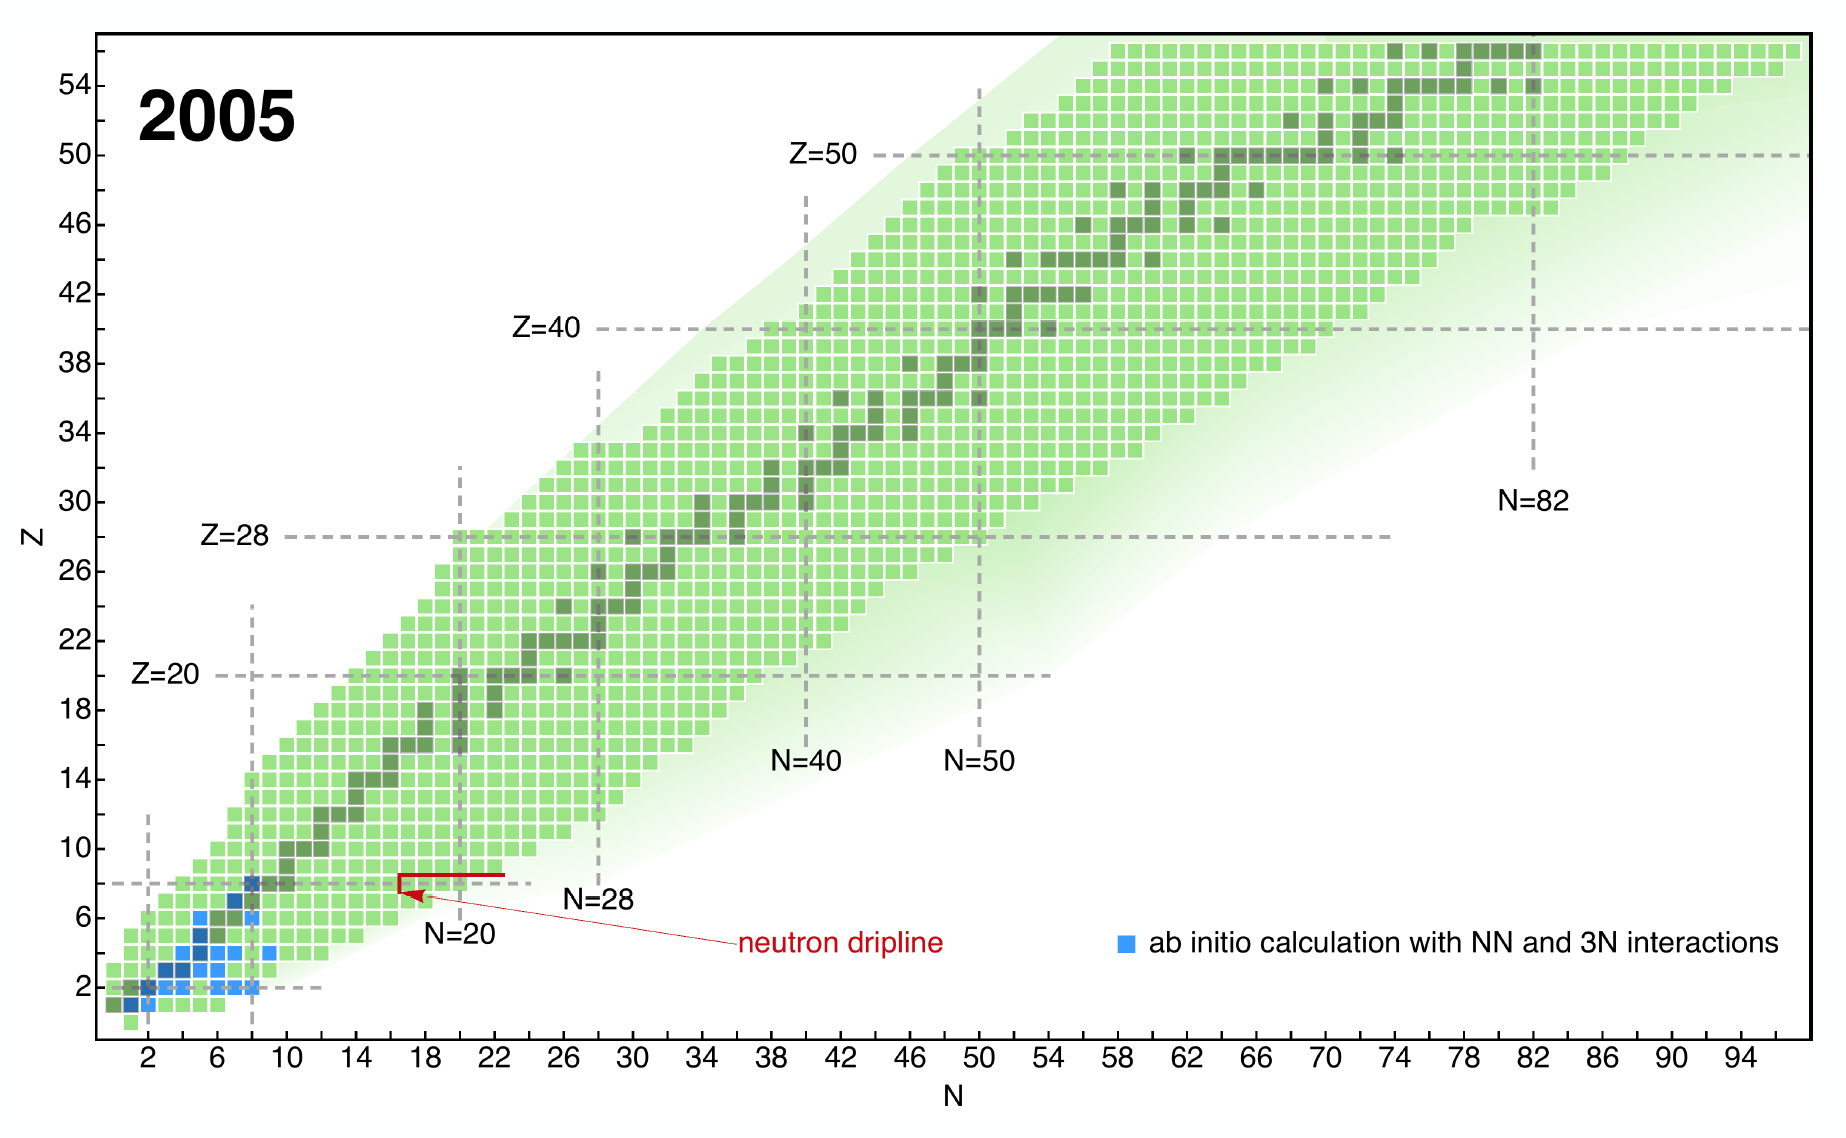
\includegraphics[width=.99\linewidth]{Figures/abinitio2005.png}
   \caption{   \label{fig:abinitio2005} }
\end{subfigure}%
\begin{subfigure}[t]{.5\textwidth}
\centering
  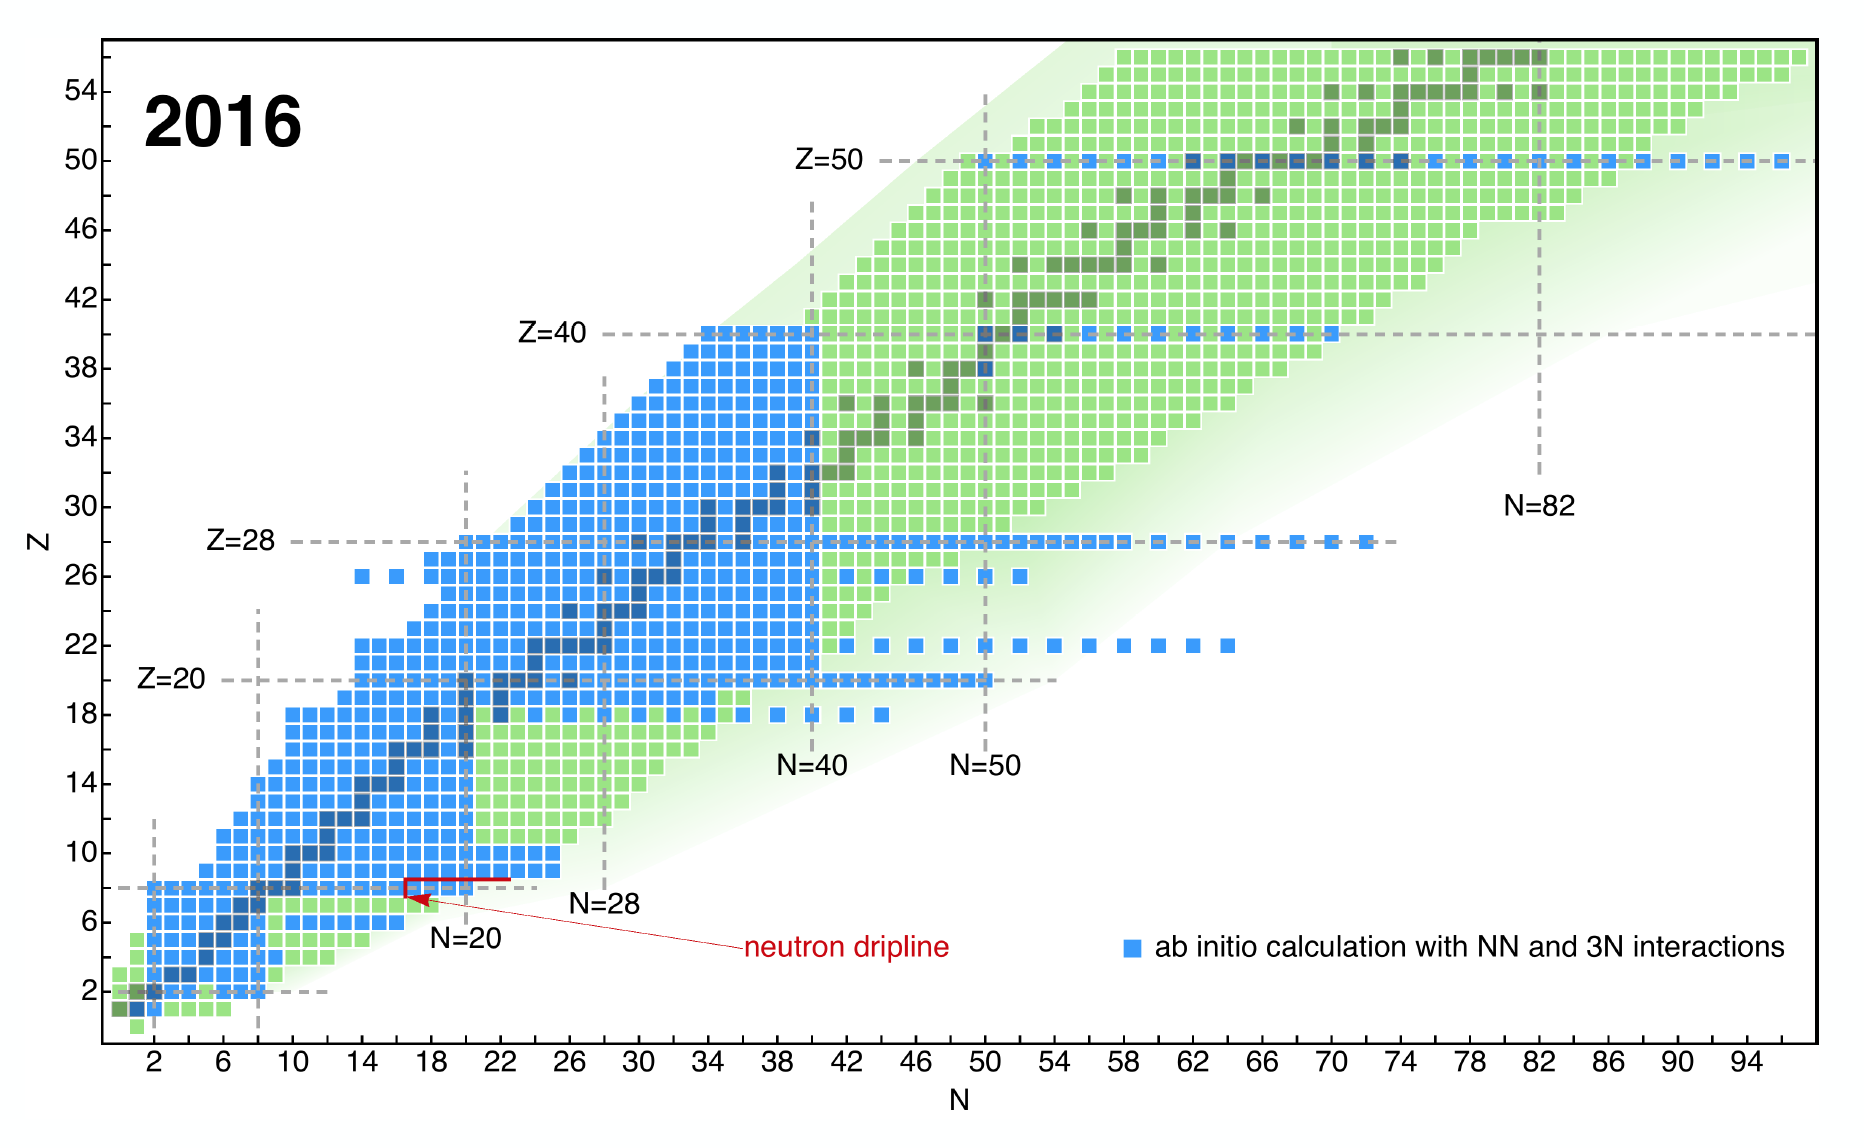
\includegraphics[width=.99\linewidth]{Figures/abinitio2016.png}
   \caption{\label{fig:abinitio2015}}
\end{subfigure}
\caption{\label{fig:abinitio}The chart of nuclides and the reach of \emph{ab initio} calculations in (a) 2005 and (b) 2016. Nuclei for which \emph{ab initio} calculations exist are highlighted in blue. Note that the figure is for illustrative purposes only, and is based on the authors' non-exhaustive survey of the literature.}
\end{figure}

The recent progress in many-body theories for nuclei are also
intimately linked with the determination and our understanding of the
equation of state (EoS) for nuclear matter.  Bulk nucleonic matter is
interesting for several reasons. The EoS of neutron matter, for
instance, determines properties of supernova explosions and neutron
stars and it relates the latter to neutron radii in atomic
nuclei. Likewise, the compressibility of nuclear matter is probed in
isoscalar giant monopole excitations, and the symmetry energy of
nuclear matter is related to the difference between proton and neutron
radii in atomic nuclei.

The developments of nuclear Hamiltonians from EFT, combined with
improved few- and many-body theories, has prepared the ground for
systematic studies of nuclear systems. The methodological and
algorithmic advances seen during the last decade allow for controlled
calculations (a high-resolution description) of nuclear properties. In
spite of these developments there are still several unsettled aspects
with nuclear Hamiltonians derived from EFT, ranging from a proper
understanding of three- and many-nucleon forces to the link with the
underlying theory of the strong force.

We are however now in a situation where progress in Lattice Quantum
Chromodynamics (LQCD) \cite{lqcd1,lqcd2} allows us to link
theoretically EFT derived Hamiltonians with LQCD calculations. The
LQCD calculations are presently performed away from the physical
masses of the constituents and the future challenges involve
developing the capabilities to perform calculations at both the
physical point, as well as away from the physical point, using lattice
spacings and volumes that can match EFT calculations.  This will allow
us to link properly LQCD, via EFT based Hamiltonians, with few- and
many-body theories used to study nuclear systems, providing thereby a
theoretical platform for understanding nuclear systems in terms of the
underlying theory for the strong force, as shown schematically in the
figure here.

\begin{figure}[hbtp]
\begin{center}
  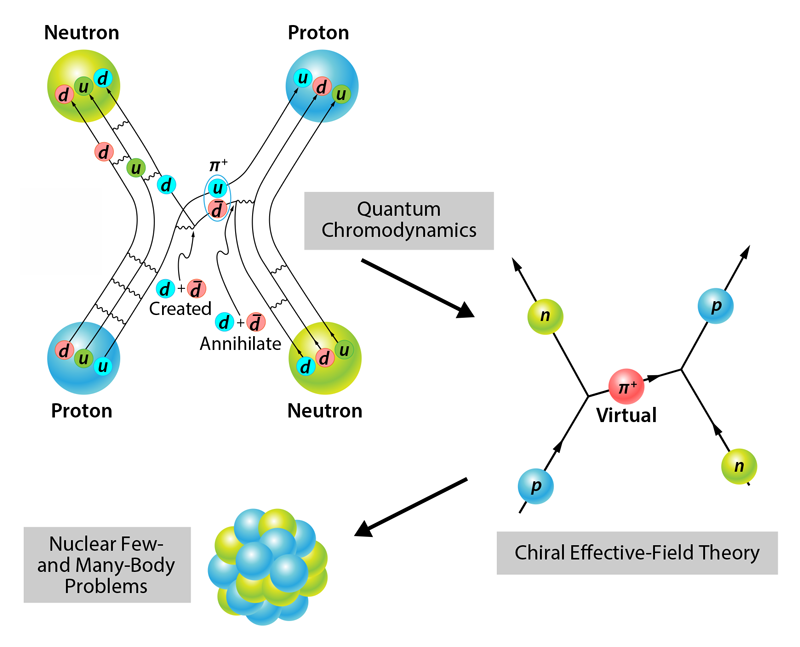
\includegraphics[width=.6\linewidth]{Figures/manybody.png}
\end{center}
\caption{A first principle approach to nuclei and nuclear matter, linking QCD with few- and many-body methods.}
\end{figure}


\subsection{Aims}

The various few- and many-body methods mentioned above allow for
controlled approximations and provide a computational scheme which
accounts for successive corrections in a systematic way.

However, all these methods face in some form or the other the problem
of an exponential growth in dimensionality. For a system of $P$
fermions which can be placed into $N$ levels, the total number of
basis states are given by
\[ \left(\begin{array}{c}N\\P\end{array}\right).  \]

The dimensional curse means that most quantum mechanical calculations
on classical computers have exponential complexity and therefore are
very hard to solve for larger systems.  If we wish to study for
example nuclei close to the limit of stability, the increased degrees
of freedom (both in terms of possible excitations as well as the
inclusion of at least two- and three-body Hamiltonians) pose severe
challenges to essentially all existing classical many-body methods.
On the other hand, a so-called quantum computer, a particularly
dedicated computer, can improve greatly on the size of systems that
can be simulated, as foreseen by Feynman
\cite{feynman1982,feynman1986}. A quantum computer does not need an
exponential amount of memory to represent a quantum state.  The basic
unit of information for a quantum computer is the so-called qubit or
quantum bit. Any suitable two-level quantum system can be a qubit, but
the standard model of quantum computation is a model where two-level
quantum systems are located at different points in space, and are
manipulated by a small universal set of operations.  These operations
are called gates in the same fashion as operations on bits in
classical computers are called gates.

The aim of this project/proposal is thus to explore and develop
algorithms based on quantum computing in order to study nuclear
systems. The first aim is to implement these algorithms on classical
computers utilizing state-of-the art technologies with both CPUs and
GPUs. We will in particular focus on quantum algorithms that can be
applied to

\begin{itemize}
\item Lattice QCD simulations of quantum field theories, with the aim to perform calculations at the physical point with relevant lattice spacings. 
\item Develop theory that allows for hybrid and multiscale simulations of LQCD and EFT on the lattice, linking thereby quark and gluonic degrees of freedom with nucleons and pions as effective degrees of freedom.
\item The link between LQCD and lattice EFT will also explore quantum machine learning algorithms, using LQCD results and experimental data on few-nucleon systems to constrain Hamiltonians for few- and many-body methods. 
\item With the pertinent effective Hamiltonians, including two- and three-body forces from EFT, we aim at developing quantum algorithms for studying nuclear few- and many-body problems. The feasibility of these algorithms will be compared to existing many-body methods like Coupled Cluster theory and in-medium Similarity Renormalization Group approaches on classical high-performance computing facilities 
\end{itemize}



\paragraph{Strategic relevance}

To understand why matter is stable, and thereby shed light on the
limits of nuclear stability, is one of the overarching aims and
intellectual challenges of basic research in nuclear physics. To
relate the stability of matter to the underlying fundamental forces
and particles of nature as manifested in nuclear matter, is central to
present and planned rare isotope facilities such as the DOE facility
FRIB under construction at Michigan State University.

To understand the stability of nuclear matter in order to interpret
the wealth of data that will come from facilities like FRIB, requires
theoretical methods that span many energy and length scales\footnote{A
  description of properties of nuclei and neutrons stars in terms of
  hadronic degrees of freedom spans over 19 orders of magnitude in
  length scale, from approximately the $10^{-15}$ m of the proton and
  neutron radii to the few kilometers which determine the radius of a
  neutron star.}. To relate the theoretical interpretations with the
underlying fundamental forces poses a severe challenge to first
principle descriptions of nuclear systems.  The theoretical modeling
of nuclear matter requires thus a multiscale approach, where different
degrees of freedom are present. Exploring algorithms based on quantum
computing and present and future high-performance computing facilities
is an essential part of our efforts to understand properly nuclear
systems.


\section{Proposed Research and Methods}

\subsection{Work Package 1 (WP1): Quantum Simulation Algorithms}

{\bf Lead Scientists: Patrick Coles (LANL) Matthew Hirn (MSU)}
\textbf{(1) Introduction} \tab The answers to many important scientific questions rely on computer simulations. Galactic evolution, weather patterns, drug discovery, and many-body physics all require high-performance computational techniques. Current computers are fundamentally limited by physical restrictions on transistor sizes---Moore's law is failing. To answer critical questions at the forefront of science, new models of computation need to be developed.


Among several promising candidates for future computing technologies (probabilistic \& neuromorphic computing, tensor \& graphical processing units, etc.), quantum computers (QCs) are one of the most exciting. For certain problems, algorithms for QCs (quantum algorithms/QAs) can provide exponential speedups over the best algorithms for current computers (for example, the quantum Fourier transform). With future QCs, such algorithms will enable us to compute in hours what would currently take years. However, current QCs are noisy and have not yet demonstrated clear advantage over classical computers. To do this, we must redesign existing QAs to counteract the noise of current QCs. For the long-term, we must design new QAs to expand the problem set future QCs can efficiently solve.


I propose to use machine learning (ML) to help (re)design QAs. This exciting new idea has been explored in two seminal papers [1, 2] and my own research [3]. ML can redesign existing algorithms for current/near-term QCs and design new algorithms for future QCs.


\textbf{(2) Preliminary work} \tab ML has been used to design QAs for mathematical functions, a result that provides important subroutines for other QAs [1]. ML has also been used to design a QA for computing quantum state overlap [2]. In collaboration with the authors of [2], I used this result to design a new QA for matrix diagonalization (pre-print at [4]).

Additionally, I used ML to redesign several known QAs for current QCs. This work has been published in a pre-print [3] that shows, e.g., the quantum Fourier transform (QFT) redesigned to the hardware constraints of ``ibmqx4'' (a current five-qubit QC). Our redesigned algorithm is more robust to noise/errors on ibmqx4 than the standard QFT algorithm.


\textbf{(3) Proposed work} \tab I propose to expand on my prior work to use ML to redesign QAs for near-term QCs (see 3.1) and design new QAs for future QCs (see 3.2). A quantum algorithm $\mathcal{A}$ is defined by a set of $N$ gates $\mathcal{A} = \{ G_i(k_i, \theta_i)\}_{i = 1}^{N}$ that describe a unitary matrix. Here, $G_i$ is the $i$th gate that acts on qubits indexed by $k_i$, and $\theta_i$ denotes internal gate parameters.

\textbf{(3.1) Algorithm redesign for near-term QCs} \tab I will use a ``cost-driven'' method to optimally redesign QAs for current/near-term QCs. Optimal algorithms need to contain as few gates as possible (due to noise), and only a limited set of gates can be implemented on current QCs. Despite this, current QCs have been used to compute the deuteron binding energy in nuclear physics, compute ground-state energies of small molecules in chemistry, and (a result of my own research [5]) learn decision boundaries for classification problems in data science. My proposed work will increase possible problem sizes (bigger nuclei/molecules/etc.) and reduce errors by redesigning QAs to have fewer gates and added ``noise-adjusting'' gates.


My proposed method works as follows. Let $\mathcal{U}$ be a known QA, $\mathcal{Q}$ a current/near-term QC, and $\mathcal{Q}_G$ the set of gates that can be implemented on $\mathcal{Q}$. The goal is to design a new algorithm, $\mathcal{A}$, that produces the same output as $\mathcal{U}$ but with fewer gates. We first initialize a guess for our trainable algorithm $\mathcal{A}$ with all gates $G_i$ from $\mathcal{Q}_G$. We then evaluate the cost $C(\mathcal{A}, \mathcal{U}) = || \mathcal{A} -  \mathcal{U} ||$ for a given matrix norm $|| \cdot ||$. The parameters $\{G_i(\theta_i), k_i\}$ in $\mathcal{A}$ are then iteratively adjusted to minimize the cost. When the cost is exactly (approximately) zero, we learn an exact (approximate) algorithm. Using similar methods in [3], I have redesigned QAs with significantly fewer gates compared to standard \textit{quantum compiling} methods, which only locally translate individual gates into $\mathcal{Q}_G$. Additionally, by training $\mathcal{A}$ in the presence of noise, our redesigned QAs add in gates to adjust for noise. Algorithms with fewer gates and noise-adjusting gates will enable more/larger problems to be solved on near-term QCs.


My proposed work will use this method to optimally redesign QAs for simulating fermionic systems on ``ibmqx5'' (a current sixteen-qubit QC). This work will enable more accurate and longer simulations of Hamiltonian evolution for many chemical systems. As QCs scale to larger sizes, my proposed method could revolutionize quantum chemistry and drug discovery.

\textbf{(3.2) Algorithm design for future QCs} \tab I will use a ``data-driven'' method to design new QAs for future QCs. The goal is to design a new QA $\mathcal{A}$ for some function $f$, which could be anything from computing quantum state overlap to a mathematical operation like integration. At a low-level, however, all such functions $f$ map bit-strings to bit-strings. %Designing new QAs is key to discovering the additional problems QCs can efficiently solve.

My proposed method works as follows. First, we pick a number of qubits $n$ and evaluate $f$ (using a classical computer) on bit-strings $x_j$. This provides training data $y_j = f(x_j)$, where $j = 1, ..., D$. We then train over the parameters $\{G_i(\theta_i), k_i\}$ in our algorithm $\mathcal{A}$ to minimize the cost $\sum_{j = 1}^{D} ||y_j - \mathcal{A}(x_j)||^2$. Then, we repeat this process for multiple $n$. After, we analyze the learned algorithms to gain insight from the quantum gates that compute $f$ on multiple problem sizes. Using pattern matching or motif recognition, we can deduce a new QA.

A similar approach was used in [2] to learn a new QA for computing state overlap. My proposed work will design new QAs for computing quantum entropies of quantum states. Such QAs, currently unknown, would be extremely useful for characterizing quantum states produced by, e.g., simulation algorithms on QCs. These functions fit well into my data-driven method because they can be computed classically \& scale naturally to multiple problem sizes. %Such QAs may provide speedups over classical algorithms because of the inherent ``quantum nature'' of quantum entropies.




\textbf{(4) Challenges} \tab In both methods, numerical optimization over the parameters $\{G_i(\theta_i), k_i)\}$ is challenging for large algorithm sizes. To overcome this, we can introduce an algorithm ``ansatz,'' or structure, to eliminate the $k_i$ and even $G_i$ parameters. Additionally, for the cost-driven method, we can train over ``sub-algorithms'' (subsets of gates) to limit the large search space while still exploring a larger space than other quantum compiling methods. %Picking a good initial guess for $\mathcal{A}$ and using a ``good'' norm $|| \cdot ||$ are both crucial for training.

For the data-driven method, deciding which gates to include in training is an open question. Further research is needed to identify the necessary number of training data points (i.e., the $D$ above). Methods from active learning can significantly reduce $D$ for large algorithm sizes.

\textbf{(5) Intellectual merit} The idea of ML for QA design has demonstrated initial success in seminal papers [1, 2] and my own research [3]. The cost-driven method searches a more expansive space than standard quantum compiling methods to produce more optimal and more robust QAs. This method could redesign any known QA for any given QC.
Methods for designing QAs for future QCs do not exist. My proposed data-driven method could produce many new QAs with applications in many fields. The recent success of this approach in [2] necessitates further study. My knowledge of both ML and QAs is ideal for these methods.

\textbf{(6) Broader impact} \tab This research will significantly increase what is possible with near-term QCs and produce new algorithms for future QCs. Both will improve our understanding of the power of QCs, which have the potential to answer some of the most important scientific questions of the 21st century. Powerful QAs could impact society outside of academia as well---e.g., efficient chemistry could discover new drugs that vastly improve human health.


The time line for WP1 is summarized in the table here:
\begin{footnotesize}
\begin{center}
\begin{tabular}{|l|c|c|c|c|c|c|c|c|c|c|c|c|}
\hline
\multicolumn{1}{|l}{Milestones } & \multicolumn{4}{|c|}{ 2020 } & \multicolumn{4}{c|}{ 2021 } & \multicolumn{4}{c|}{ 2022 } \\
\hline
Topic 1 &$\bullet$ &$\bullet$ &$\bullet$ &$\bullet$ & & & & & & & &  \\
\hline
Topic 2 & & &$\bullet$ &$\bullet$ &$\bullet$ &$\bullet$ & & & & & &  \\
\hline
Topics 3 & & & & $\bullet$ &$\bullet$ &$\bullet$ &$\bullet$ & & & & &  \\
\hline
Topic 4 & &$\bullet$ & & & &$\bullet$ & & & &$\bullet$ & &  \\
\hline
\end{tabular}
\end{center}
\end{footnotesize}

\subsection{Work Package 2 (WP2): Lattice Quantum ChromoDynamics (QCD) and Quantum Information Theories}
{\bf Lead Scientists: Alexei Bazavov (MSU), Huey-Wen Lin (MSU) and Andrea Shindler (MSU)}


The time line for WP2 is summarized in the table here:
\begin{footnotesize}
\begin{center}
\begin{tabular}{|l|c|c|c|c|c|c|c|c|c|c|c|c|}
\hline
\multicolumn{1}{|l}{Milestones } & \multicolumn{4}{|c|}{ 2020 } & \multicolumn{4}{c|}{ 2021 } & \multicolumn{4}{c|}{ 2022 } \\
\hline
Topic 1 &$\bullet$ &$\bullet$ &$\bullet$ &$\bullet$ & & & & & & & &  \\
\hline
Topic 2 & & &$\bullet$ &$\bullet$ &$\bullet$ &$\bullet$ & & & & & &  \\
\hline
Topics 3 & & & & $\bullet$ &$\bullet$ &$\bullet$ &$\bullet$ & & & & &  \\
\hline
Topic 4 & &$\bullet$ & & & &$\bullet$ & & & &$\bullet$ & &  \\
\hline

\end{tabular}
\end{center}
\end{footnotesize}

\subsection{Work package 3 (WP3): Quantum state preparation and dynamics}
{\bf Lead Scientists: Dean Lee (MSU)}

The research activity of Dean Lee focuses on developing new algorithms for quantum state preparation and time evolution that are sufficiently robust to operate on noisy near-term devices.  These include both digital quantum computers and analog quantum simulators.  The problems we address are designed to probe correlations in nuclear structure, the spectrum of nuclear energy levels, transition matrix elements, and the dynamics of nuclear scattering and reactions.  Graduate  student Jacob Watkins has worked on the topics presented in this proposal and funds would be used to support his continuing research in quantum computing applied to nuclear physics. 





\subsubsection{Variational adiabatic evolution}

In order to perform calculations of the properties of nuclear systems
via quantum computing, we need to be able to prepare quantum states in
an eigenstate of the nuclear Hamiltonian. The method of adiabatic
evolution is one approach to quantum state preparation
\cite{Farhi:2000a}.  The adiabatic theorem tells us that if we start
in an eigenstate of some time-dependent Hamiltonian $H(t)$, then we
remain in an eigenstate of $H(t)$ so long as the time dependence is
sufficiently slow and we do not pass through level crossings.  Let us
start with some simple Hamiltonian $H_z$ whose ground state
$\ket{\phi^0_z}$ can be prepared simply using single qubit gate
operations. Suppose we want to produce the ground state
$\ket{\phi^{0}_\odot}$ for some nontrivial Hamiltonian $H_\odot$.  We
can define a time-dependent Hamiltonian $H(t)$ so that $H(0)=H_z$ and
$H(\tau)=H_\odot$.  If the time dependence is sufficiently slow and we
do not pass through any level crossings, then we obtain an accurate
representation of $\ket{\phi_\odot}$ after reaching time $t = \tau$,

\begin{equation}
\ket{\phi_\odot^0} = T \exp\left[-i\int_0^\tau H(t) dt \right]\ket{\phi_z^{0}}.
\end{equation}  
In practice, however, decoherence on near-term devices means that the
amount of time evolution is severely limited.  This problem is
substantially ameliorated for an analog quantum simulator.  However,
there remains a general problem of dealing with the errors generated
by imperfect adiabatic evolution.

The strategy of variational adiabatic evolution is to produce a
subspace of states corresponding to different time-dependent
Hamiltonians $H_{n}(t)$.  We construct the time-evolved state
$\ket{\psi_n} = U_n\ket{\phi_z^0}$, where $U_n$ is
\begin{equation}
U_n = T \exp\left[-i\int_0^\tau H_n(t) dt \right] \label{adiabatic}.
\end{equation}
 This unitary operation can be implemented in small time steps using
 the Trotter approximation. In order to compute the inner product
 $\braket{\psi_n|\psi_m}$ and amplitude
 $\braket{\psi_n|H_\odot|\psi_m}$ we use one auxiliary qubit.  We
 initialize the auxiliary qubit as $\ket{0}$ while the main system is
 prepared in the state $\ket{\phi_z^0}$.  We perform a Hadamard
 transform on the auxiliary qubit and implement controlled unitary
 gate operations to obtain
\begin{equation}
\ket{0}\ket{\phi_z^0} \rightarrow (1/\sqrt{2}\ket{0} +1/\sqrt{2}\ket{1})\ket{\phi_z^0}
\rightarrow 1/\sqrt{2}\ket{0}U_n\ket{\phi_z^0} +1/\sqrt{2}\ket{1}U_m\ket{\phi_z^0}.
\end{equation}
In order to compute the inner product $\braket{\psi_n|\psi_m},$ we
measure the expectation value of $\sigma_x$ plus $i$ times $\sigma_y$
upon the auxiliary qubit.  In order to compute the amplitude
$\braket{\psi_n|H_\odot|\psi_m}$, we measure measure the expectation
value of $\sigma_x \otimes H_\odot$ plus $i$ times $\sigma_y \otimes
H_\odot$.  Equipped with the inner products $\braket{\psi_n|\psi_m}$
and amplitudes $\braket{\psi_n|H_\odot|\psi_m}$, we can now solve for
the variational ground state of $H_\odot$ in the subspace spanned by
the vectors $\ket{\psi_n}$.

We propose to test the variational adiabatic evolution method for a
particle on a one-dimensional lattice of length $2L+1$ with an
attractive short-range potential at the center of the chain.  We can
write the pieces of the Hamiltonian as

\begin{align}
H_z &= \sigma_z^{(L)}, \\
H_{\rm even} &= \frac{1}{2} \sum_{n=0,2,\cdots,2L-2} [\sigma_x^{(n+1)}\sigma_x^{(n)}
+ \sigma_y^{(n+1)}\sigma_y^{(n)}], \\
H_{\rm odd} &= \frac{1}{2} \sum_{n=1,3,\cdots,2L-1} [\sigma_x^{(n+1)}\sigma_x^{(n)}
+ \sigma_y^{(n+1)}\sigma_y^{(n)}], \\
H_\odot &= H_z + H_{\rm even} + H_{\rm odd}.
\end{align}
We note that all of the terms in $H_{\rm even}$ commute with each other and all of the terms in $H_{\rm odd}$ commute with each other.  This simplifies the unitary time evolution.  In order to describe the physics of a single particle, we consider the linear space where exactly one qubit is in the $\ket{1}$ state and the remaining $2L$ qubits are in the  $\ket{0}$ state.  For $L_t$ time steps and total evolution time $\tau$, we define the time interval $dt=\tau/L_t$.  We let the unitary operator at time step $n_t$ be
\begin{equation}
U(n_t,L_{t},dt) = \exp(-iH_{\rm odd}n_tdt/L_t)\exp(-iH_{\rm even}n_tdt/L_t)\exp(-iH_ zdt).   
\end{equation} 
We will work with the evolved state,
\begin{equation}
\ket{\psi,\tau,L_t} = U(n_t,L_{t},dt) \cdots U(2,L_{t},dt)U(1,L_{t},dt)\ket{\phi_z^0}. 
\end{equation}

We have done some preliminary work to show that this method appears
viable. The exact ground state energy of $H_\odot$ in the limit $L
\rightarrow \infty$ is $-\sqrt{2}$.  For $L = 100$ the energy to four
significant digits is $-1.414$. If we use the parameters $\{\tau =
1.0,L_t = 4\},$ we find that the energy expectation value of
$\ket{\psi,\tau,L_t}$ is $-0.973$.  This is not an accurate estimate
of the ground state energy, but as good as one might achieve with
current digital quantum computing technology.  If we now apply
variational adiabatic evolution with two different trajectories,
$\{\tau = 1.0,L_t = 4\}$ and $\{\tau = 1.5,L_t = 4\},$ we get a
variational energy of $-1.364$.  We see that there is significant
improvement as the variational approach is able to remove some
contamination from other low-lying energy states. If we now apply
variational adiabatic evolution with three different trajectories,
$\{\tau = 1.0,L_t = 4\}, \{\tau = 1.5,L_t = 4\},$ and $\{\tau =
2.0,L_t = 4\}$, we get a variational energy of $-1.399$.  The method
appears to be converging rapidly with the number of variational
states.

We propose to study the convergence rate and error stabilization of
variational adiabatic evolution for our quantum particle bound to a
potential for various values of $L$.  We first analyze the system
using standard classical computing with simulation software such as
Qiskit.  We then work with our collaboration partners to implement on
digital quantum computing devices at IBM Q.  We will
compare with standard adiabatic evolution as well as the quantum
approximate optimization algorithm \cite{Farhi:2014}. We will vary the
number of particles, $N$, and vary the width of the trapping potential
in $H_z$.  Our many-body system will correspond to $N$ identical
spinless fermions in a one-dimensional trap.  For $L = 40$ and $N =
20$ the number of possible quantum states will exceed $10^{11}$.

Perhaps the most important aspect of this project is error
stabilization.  The inner products $\braket{\psi_n|\psi_m}$ and
amplitudes $\braket{\psi_n|H_\odot|\psi_m}$ will suffer from noise.
The first step is to remove any systematic biases using known
extrapolation methods \cite{Kandala:2019}. For the remaining error we
apply new tools that we have recently developed for another
computational technique called eigenvector continuation
\cite{Frame:2017fah}.  The error stabilization algorithm involves
Monte Carlo simulations of the data with estimated errors included,
while throwing out trials that do not satisfy physically-motivated
conditions such as norm positivity and constraints on level ordering.
    
If we add a complex Gaussian error with width $0.05$ to each of the
inner products $\braket{\psi_n|\psi_m}$ and amplitudes
$\braket{\psi_n|H_\odot|\psi_m}$ in our previous variational
calculation with three trajectories, then our error stabilization
algorithm gives an estimate of $-1.51(24)$. If error size is reduced
to $0.02$, the estimate is $-1.46(12)$. For an error of size $0.01$
the estimate is $-1.41(7)$.  We propose to make further improvements
to the error stabilization algorithm by studying the behavior of
eigenvectors and eigenvalues under noise perturbations.  We will
investigate both the underlying theory and its practical
implementation.

\subsubsection{Spectral reconstruction and transition matrix elements}
     
Quantum phase estimation is one approach to computing the spectrum of
a Hamiltonian through real-time evolution and the inverse quantum
Fourier transform \cite{Abrams:1999}.  We propose to investigate a
different approach that can compute the low-lying excitation spectrum
of a quantum system without the use of auxiliary qubits.  The steps
are as follows.  We first prepare the state $\ket{\psi}$ using
imperfect adiabatic evolution, as we have discussed in the text
surrounding Eq.~(\ref{adiabatic}). We can write $\ket{\psi}$ as a
linear combination of eigenstates of $H_\odot$,

\begin{equation}
\ket{\psi} = \sum_n c_n \ket{\phi^n_\odot}.
\end{equation}The strategy is to prepare $\ket{\psi}$ so that the sum is dominated by only a few low-lying eigenvectors. 



Let $O$ be some Hermitian operator that does not commute with the Hamiltonian and thus induces  transitions between energy eigenstates.  For example, $O$ could be an electric multipole operator for a nuclear system. We evolve the state $\ket{\psi}$ for a sequence of equally-spaced times $t$,
\begin{equation}
\ket{\psi(t)} = \exp(-iH_{\odot}t) \ket{\psi}.
\end{equation}
We measure the expectation value of $O$ for each $t$, 
\begin{equation}
\braket{O(t)} = \braket{\psi(t)| O |\psi(t)}. 
\end{equation}
In terms of the energy eigenstates, the expectation value is 
\begin{equation}
\braket{O(t)} =   \sum_{n'}  \sum_n c^*_{n'} c_n \braket{\phi^{n'}_\odot|O|\phi^n_\odot}
e^{-i(E^{n}_\odot-E^{n'}_\odot)t},
\end{equation}
where $E^{n}_\odot$ is the energy corresponding to
$\ket{\phi^n_\odot}$.  Using a classical computer, we now calculate
the Fourier transform of $\braket{O(t)}$.  From the Fourier transform
we can extract the energy differences $E^{n}_\odot-E^{n'}_\odot$.
This gives us the excitation energies of all low-lying states with
non-negligible overlap with $\ket{\psi(t)}$.

We propose to develop the efficiency of this spectral reconstruction
technique by exploring various transition operators $O$ and various
imperfectly-evolved states $\ket{\psi(t)}$ that maximize the
transition of each excited state to the ground state.  We have done
some preliminary work to show that this method is viable for analog
quantum simulators.  As an example we consider the so-called time
fractal system of trapped ions as described in
Ref.~\cite{Lee:2019gtc}.  Similar to atomic nuclei, this system has a
rich spectrum of bound states.  The bound state energies form a
geometric sequence as a consequence of discrete scale invariance.


We consider a one-dimensional chain of ions in a radio-frequency trap
with qubits represented by two hyperfine ``clock'' states.  Such
systems have been pioneered by the Monroe group using $^{171}$Yb$^{+}$
ions \cite{Zhang:2017a,Zhang:2017b}.  Off-resonant laser beams are
used to drive stimulated Raman transitions for all ions in the trap.
This induces effective interactions between all qubits with a
power-law dependence on separation distance.  We define the vacuum
state as the state with $\sigma_z^{(n)}=1$ for all sites $n$.  We use
interactions of the form
$\sigma_x^{(n)}\sigma_x^{(n')}+\sigma_y^{(n)}\sigma_y^{(n')}$, to
achieve the hopping of spin excitations.  We then use a
$\sigma_z^{(n)}\sigma_z^{(n')}$ interaction to produce a two-body
potential felt by pairs of spin excitations, and we also consider an
external one-body potential coupled to $\sigma_z^{(n)}$.

We can view each spin excitation with $\sigma_z^{(n)}=-1$ as a bosonic
particle at site $n$ with hardcore interactions preventing multiple
occupancy.  In this language, the Hamiltonian we consider has the form

\begin{align}
H =\frac{1}{2} \sum_{n}\sum_{n'\ne n} J_{nn'}[b^{\dagger}_n b_{n'} +b^{\dagger}_{n'}
b_n] & + \frac{1}{2}\sum_{n}\sum_{n' \ne n}V^{}_{nn'}b^{\dagger}_n b_n b^{\dagger}_{n'}
b_{n'} \nonumber\\
& + \sum_{n}U^{}_{n}b^{\dagger}_n b_n+C, \label{time_fractal}
\end{align}
where $b_n$ and $b^{\dagger}_n$ are annihilation and creation
operators for the hardcore bosons on site $n$.  The hopping
coefficients $J_{nn'}$ have the form $J_{nn'} =
J_0/|r_n-r_{n'}|^{\alpha}$, where $r_n$ is the position of qubit $n$.
Similarly, the two-body potential coefficients $V_{nn'}$ have the form
$V_{nn'} = V_0/|r_n-r_{n'}|^{\beta}$.

We now add to $U_n$ a deep attractive potential at some chosen site
$n_0$ that traps and immobilizes one boson at that site.  Without loss
of generality, we take the position of that site to be the origin and
add a constant to the Hamiltonian so that the energy of the trapped
boson is zero.  We then consider the dynamics of a second boson that
feels the interactions with this fixed boson at the origin.  In order
to produce a quantum system with a geometric spectrum and discrete
scale invariance, we choose $\beta=\alpha-1$. As an example, we
consider a system with $\alpha = 2$, $\beta = 1$, $J_0 = -1$, and $V_0= -30$.  
The wave functions for the first twelve even-parity bound
states are shown in Fig.~\ref{even_wavefunctions}.  We plot the
normalized wave function for $r>0$, where $r$ is measured in lattice
units.
     

\begin{figure}
\centering
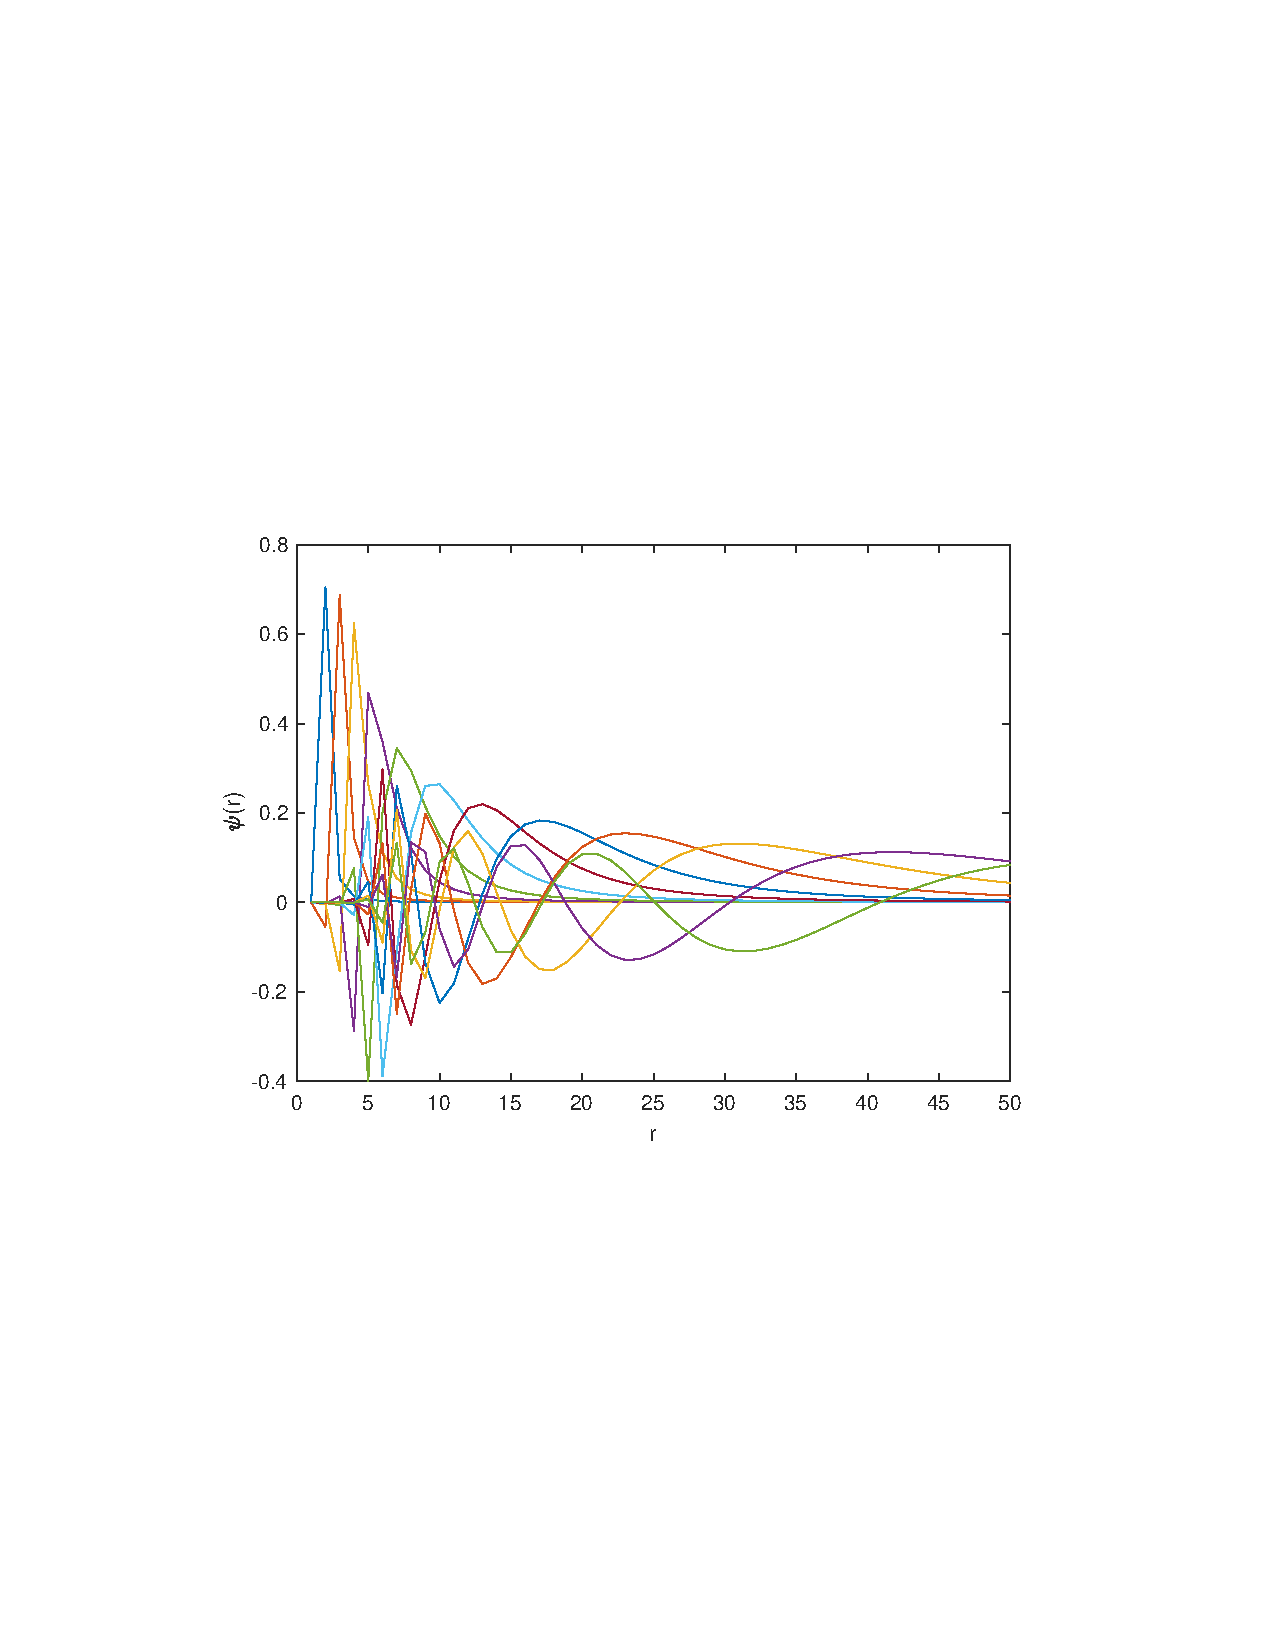
\includegraphics[width=8cm]{v30_even_wavefunctions}
\caption{Plot of the normalized wave functions
for the first twelve even-parity bound states for the case $\alpha =
2$, $\beta = 1$, $J_0 = -1$, and $V_0 = -30$.  We plot the region
$r>0$, where $r$ is measured in lattice units.}
\label{even_wavefunctions}
\end{figure}

We propose to reconstruct the excitation spectrum of the time fractal
system using transition operators of the form $b^{\dagger}_n b_n$ for
some particular value of $n$.  This is analogous to the single-nucleon
charge density operator.  In addition to the energy differences
$E^{n}_\odot-E^{n'}_\odot$, we can also extract $c^*_{n'} c_n
\braket{\phi^{n'}_\odot|O|\phi^n_\odot}$.  Given the fact that $\sum_n
|c_n|^2=1,$ this provides a lower bound on the magnitude of the
transition matrix element,
$|\braket{\phi^{n'}_\odot|O|\phi^n_\odot}|$. We propose to study
different imperfectly-evolved states $\ket{\psi(t)}$ to generate many
different coefficients $c_n$ and thus estimate the magnitude of the
transition matrix elements
$|\braket{\phi^{n'}_\odot|O|\phi^n_\odot}|$.
  
\subsubsection{Scattering, reactions, and few-body dynamics}

We propose to study the real-time dynamics of colliding particles and
bound states.  The goal is to provide data from analog quantum
simulators that can be used to benchmark state-of-the-art tools used
for nuclear scattering and reactions such as the adiabatic projection
method \cite{Elhatisari:2015iga}.  For this purpose we use again the
time fractal system with Hamiltonian described in
Eq.~(\ref{time_fractal}).  In this case, however, we do not include
any trapping potential at the center.  Instead we have keep the system
uniform except for the open boundary conditions at the ends of the
trap.

We have performed preliminary work showing that we can study the
real-time dynamics of colliding particles and bound states in this
manner.  As discussed above, we define the vacuum state as the state
with $\sigma_z^{(n)}=1$ for all sites $n$.  We can view each spin
excitation with $\sigma_z^{(n)}=-1$ as a bosonic particle at site $n$
with hardcore interactions preventing multiple occupancy. If we
initialize the system with one particle at the left edge of the ion
trap, we can produce a wave packet that moves to the right and bounces
elastically off the trap boundaries. In Fig.~\ref{particle} we plot
the real-time dynamics of a single particle released from the left
edge of an $L=30$ trap.  We are plotting the particle density for
several time snapshots, with later times linearly displaced in the
vertical direction.

In a similar fashion we can initialize a dimer (two-particle) wave
packet by putting two particles on adjacent sites at the edge of the
ion trap. In Fig.~\ref{dimer_particle} we plot the real-time dynamics
of a dimer and particle released from the left and right edges
respectively of an $L=30$ trap.  We are plotting the particle density
for several time snapshots, with later times linearly displaced in the
vertical direction.
 

  The collisions between any $N_1$-body state and $N_2$-body state can
  be realized in this trapped ion system.  We propose to study how to
  extract scattering observables from real-time processes on analog
  quantum simulators.  For elastic scattering we propose to determine
  reflection and transmission coefficients.  For inelastic scattering
  we would also like to determine transfer and breakup probabilities
  for both inclusive and exclusive process. We propose to produce
  high-quality scattering and reaction data that can be used to
  benchmark the adiabatic projection method currently being used for
  nuclear scattering and reactions in lattice effective field theory.

\begin{figure}
\centering
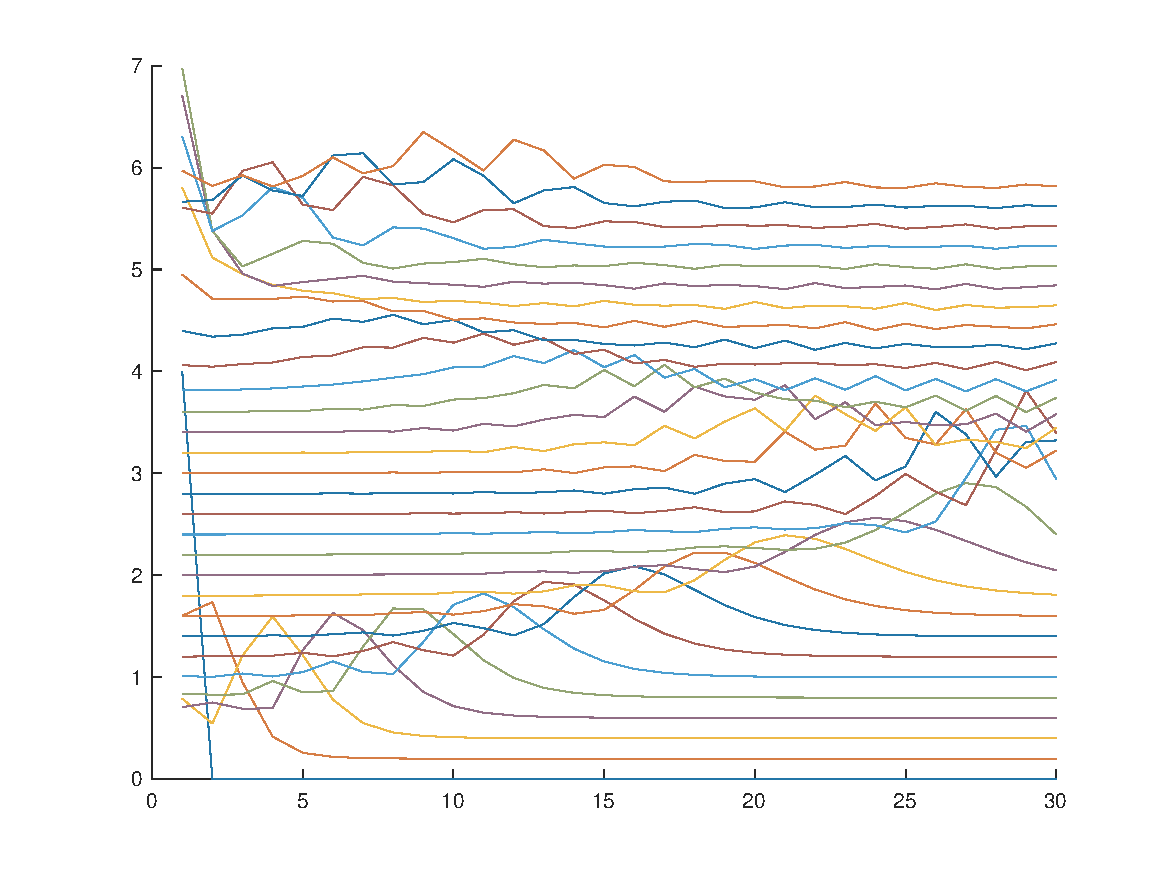
\includegraphics[width=8cm]{particle_1}
\caption{Plot of the real-time dynamics of a single particle released from the left edge of an $L=30$ trap.  We are plotting the particle density for several time snapshots, with later times linearly displaced in the vertical direction.}
\label{particle}
\end{figure}
 
\begin{figure}
\centering
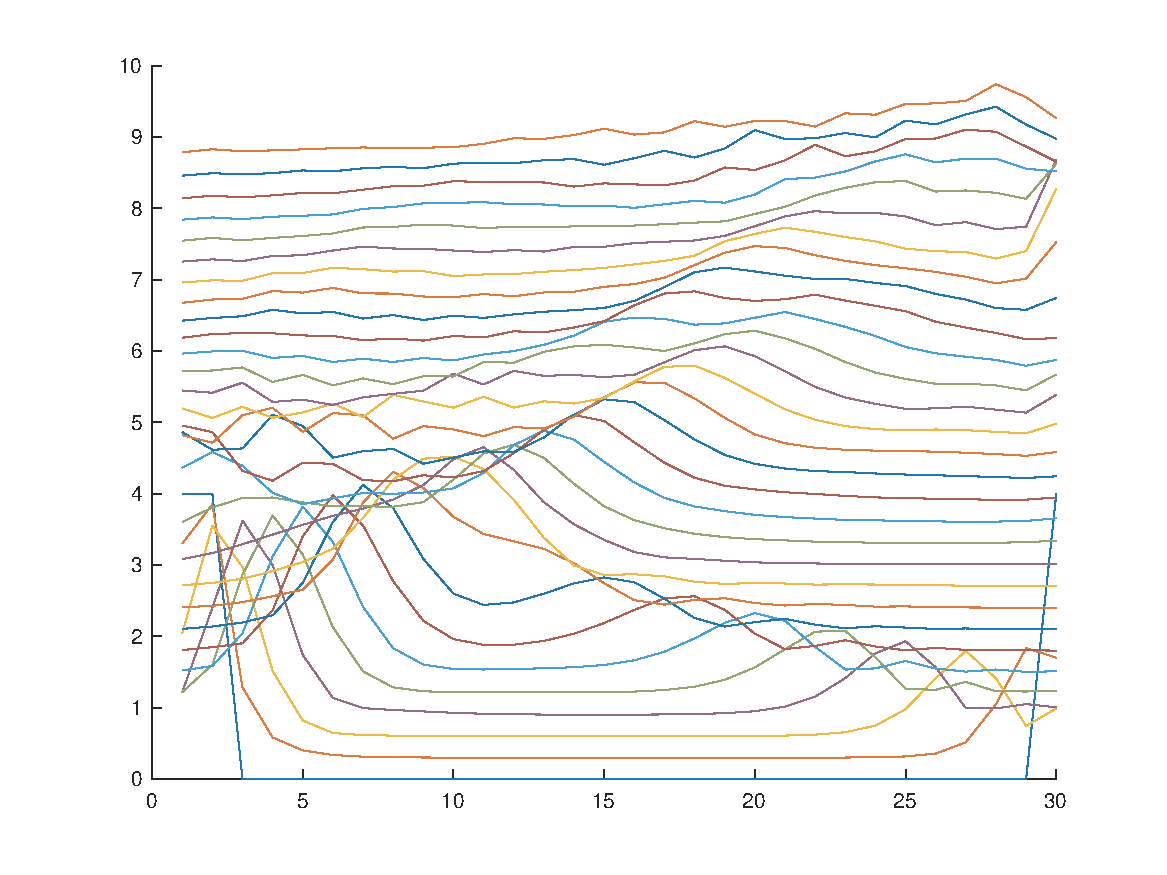
\includegraphics[width=8cm]{dimer_particle_1}
\caption{Plot of the real-time dynamics of a dimer and a single particle released from the left and right edges respectively of an $L=30$ trap.  We are plotting the particle density for
several time snapshots, with later times linearly displaced in the vertical
direction.}
\label{dimer_particle}
\end{figure}

 The time line for the development of the various elements of WP3 is
\begin{footnotesize}
\begin{center}
\begin{tabular}{|l|c|c|c|c|c|c|c|c|c|c|c|c|}
\hline
\multicolumn{1}{|l}{Milestones } & \multicolumn{4}{|c|}{ 2020 } & \multicolumn{4}{c|}{ 2021 } & \multicolumn{4}{c|}{ 2022 } \\
\hline
Variational adiabatic evolution &$\bullet$ &$\bullet$ &$\bullet$ &$\bullet$ & & & & & & & &  \\
\hline
Spectral reconstruction & & & $\bullet$ &$\bullet$ &$\bullet$ &$\bullet$ & & & & & &  \\
\hline
Transition matrix elements & & & & & $\bullet$ &$\bullet$ &$\bullet$ &$\bullet$ & & & &   \\
\hline
Scattering and reactions & & & & & & & & & $\bullet$ &$\bullet$ &$\bullet$ &$\bullet$ \\
\hline

\end{tabular}
\end{center}
\end{footnotesize}

\subsection{Work Package 4 (WP4): Nuclear structure, Finite Nuclei and Infinite Nuclear Matter}
{\bf Lead Scientists: Scott Bogner (MSU), Heiko Hergert (MSU) and Morten Hjorth-Jensen (MSU)}
\paragraph{Simulation of Many-Body Hamiltonians}

Given a Hamiltonian in second-quantized form
\begin{align*}
H=\sum_{pq}h_{pq}\dagg{a_p}a_q+\sum_{pqrs}h_{pqrs}\dagg{a_p}\dagg{a_q}a_sa_r
\end{align*}
for example, one can use a quantum computer to estimate the energy eigenvalues of the Hamiltonian $E_n$ where $H\ket{\psi_n}=E_n\ket{\psi_n}$. First, one maps the Hamiltonian to quantum gates via a mapping such as the Jordan-Wigner transformation
\begin{align*}
\dagg{a_i}&=\sigma_z^{\otimes i-1}\otimes\sigma_+\otimes\mathbb{I}^{\otimes n-i} \\
\nonumber
a_i&=\sigma_z^{\otimes i-1}\otimes\sigma_-\otimes\mathbb{I}^{\otimes n-i}
\end{align*}
The most efficient mapping is still unknown.
Then, one must approximate the time-evolution operator
\begin{align*}
U=e^{-iHt/\hbar}=e^{-i\sum_kH_kt/\hbar}
\end{align*}
using an approximation such as Suzuki-Trotter
\begin{align*}
e^{A+B}=\lim_{n\to\infty}\left(e^{A/n}e^{B/n}\right)^n
\end{align*}
Which approximation to use for a given problem is an active area of research.
Next, one maps the time-evolution operator into quantum circuits consisting of 2-qubit gates. The mapping that results in the shortest depth quantum circuit is an open question. Finally, one plugs the quantum circuit for $U$ into the phase estimation algorithm.

This process can be used to simulating nuclear systems such as infinite matter (jellium) or be used to estimate binding energies. The theoretical expertise hear at the NSCL/FRIB is extremely helpful in setting up the problems in such a way that they can be most efficiently solved by a quantum computer.

In the near-term, the variational quantum eigensolver algorithm is best suited to solve problems. It is a hybrid quantum-classical algorithm that is based on the variational principle of quantum mechanics
\begin{align*}
\bra{\psi(\theta)}H\ket{\psi{\theta}}\geq E_0
\end{align*}
where $E_0$ is the ground state. The quantum computer is used to prepare an initial state that one guesses and measure the expectation value of the Hamiltonian in that state. The initial state is then slightly varied by a small change in the parameters $\theta$ and the expectation value is measured again. The classical computer computes some norm of the difference between the iterations of the expectation values and stops when this norm is sufficiently small. The algorithm will converge to the ground state energy of the Hamiltonian. The excited energies can be calculated by shifting the Hamiltonian and repeating the algorithm.

The time line for WP4 is summarized in the table here:
\begin{footnotesize}
\begin{center}
\begin{tabular}{|l|c|c|c|c|c|c|c|c|c|c|c|c|}
\hline
\multicolumn{1}{|l}{Milestones } & \multicolumn{4}{|c|}{ 2020 } & \multicolumn{4}{c|}{ 2021 } & \multicolumn{4}{c|}{ 2022 } \\
\hline
Topic 1 &$\bullet$ &$\bullet$ &$\bullet$ &$\bullet$ & & & & & & & &  \\
\hline
Topic 2 & & &$\bullet$ &$\bullet$ &$\bullet$ &$\bullet$ & & & & & &  \\
\hline
Topics 3 & & & & $\bullet$ &$\bullet$ &$\bullet$ &$\bullet$ & & & & &  \\
\hline
Topic 4 & &$\bullet$ & & & &$\bullet$ & & & &$\bullet$ & &  \\
\hline

\end{tabular}
\end{center}
\end{footnotesize}

\subsubsection{Broader Impacts}

The academic environment at MSU provides numerous opportunities for
the PIs to attract bright young people to high-level research in
nuclear physics. For example, the theory group at the NSCL is very
active in mentoring undergraduate students in the NSF sponsored
Research Experience for Undergraduates (REU) program in the summer
months, with the PIs successfully supervising two REU students over
the past three years. Many of the projects in this proposal can be
tested in prototype toy-model problems that manage to simultaneously
i) illustrate cutting-edge concepts to the student at a technical
level appropriate for an undergraduate physics major, and ii) benefit
the overall progress of the PIs' research program.

One of the primary \emph{broader impacts} of our previous NSF award,
which we will continue in the current award, is the development of an
open source library that can be used by other theorists and serve as a
educational resource for graduate students and postdocs learning about
advanced many-body methods like CC and IMSRG.  In our recent Lecture
Notes in Physics book~\cite{lnp}, we have together with our graduate
students and other colleagues, written two long chapters on the
application of the above many-methods to neutron star studies. These
chapters contain links to our codes, which are fully open source and
contain benchmark calculations as well, making thereby our science
reproducible. They can be accessed via the GitHub link
\url{https://github.com/ManyBodyPhysics/LectureNotesPhysics/tree/master/doc/src}. As
we implement the infinite matter projects described in the current
proposal (e.g., inclusion of NNN forces and approximate triples
excitations, calculation of spin-isospin response functions, etc.),
the codes in the repository will be updated accordingly.

The PIs are requesting support for three graduate students plus one
postdoc to work on the projects outlined above. The methods at the
center of this proposal are at the forefront of basic research in
many-body physics and low-energy nuclear physics.The many
collaborations of the PIs with academic institutions world wide
provides an excellent platform for developing the communication skills
of the supported students. Global collaboration, and collaboration
within the local group, requires skills in project management in order
to adequately communicate the progress of the project and to meet
deadlines. Participation in international conferences and visits at
research centers can be expected within the time period the proposed
project. This will equip the involved participants with skills in
presentation techniques.  Proper documentation, both internally and in
peer-reviewed international journals, in writing is expected. The
project is grounded in nuclear physics but there is a very large
overlap with computational science and numerical analysis. These two
complementary aspects will form a natural part of the everyday work
and therefore add to the total competence of the
participants. Naturally, this will add to the number of possible
career paths.





\subsection{Tasks}

\section{Work Package 5 (WP5): Workforce Development}

The time line for WP5 is summarized in the table here:
\begin{footnotesize}
\begin{center}
\begin{tabular}{|l|c|c|c|c|c|c|c|c|c|c|c|c|}
\hline
\multicolumn{1}{|l}{Milestones } & \multicolumn{4}{|c|}{ 2020 } & \multicolumn{4}{c|}{ 2021 } & \multicolumn{4}{c|}{ 2022 } \\
\hline
Topic 1 &$\bullet$ &$\bullet$ &$\bullet$ &$\bullet$ & & & & & & & &  \\
\hline
Topic 2 & & &$\bullet$ &$\bullet$ &$\bullet$ &$\bullet$ & & & & & &  \\
\hline
Topics 3 & & & & $\bullet$ &$\bullet$ &$\bullet$ &$\bullet$ & & & & &  \\
\hline
Topic 4 & &$\bullet$ & & & &$\bullet$ & & & &$\bullet$ & &  \\
\hline

\end{tabular}
\end{center}
\end{footnotesize}

\subsection{Mentoring Plan}

The mentoring of the graduate students postdoc located at the
FRIB/NSCL facility will be fully incorporated in the existing
mentoring program of FRIB/NSCL. At any time there are about 15
experimental and theoretical postdocs and approximately 100 graduate
students at the FRIB/NSCL. It is an ideal research environment which
will enable the graduate students and postdoc to work and interact
with students, postdocs and more senior researches with diverse
backgrounds on a daily basis. A few years ago FRIB/NSCL strengthened
and improved the mentoring of graduate students and postdocs at the
FRIB/NSCL with the appointment of an Associate Director for
Education. A formal half-year review of all postdocs was initiated. It
begins with an entry interview where the postdoc and supervisor
discuss expectations and future career plans of the postdoc guided by
a form containing standard topics and questions related to the
research activities. This initial discussion is then followed but by
similar meetings every 6 months. These reviews occur in April and
October of each year and are required and monitored by the Associate
Director for Education.  The Associate Director for Education meets
with all FRIB/NSCL postdocs on a monthly basis to keep them informed
about FRIB/NSCL related news and activities. During these meetings the
representative of the various committees also report back to the
group. Postdocs also maintain their own website, where they share
experiences, hints and collect and list job openings. Postdocs are
also encouraged to participate in activities and programs offered by
the University and the professional societies. For example, recent
postdocs have been participating in an MSU sponsored Work/Life balance
workshop and the APS professional development workshops. The FRIB/NSCL
especially focuses on career planning. Every semester two seminar
speakers are especially chosen to present a broad view of career
opportunities outside the traditional academic track. Yearly alumni
events offer additional interaction of current students and postdocs
with successful NSCL alumni in a variety of careers.  The FRIB/NSCL
alumni contact list currently contains the names of 250 alumni who
offered to be contacted by students and postdocs for career advice
(\url{http://www.nscl.msu.edu/ourlab/alumni}).  The list can be
filtered by profession and geographic distribution.  Finally, the
postdocs are an integral part of all laboratory social activities at
the NSCL which include the Tuesdays coffee and bagel, Thursdays ice
cream social, as well as summer BBQs and welcome receptions. These
activities further foster the interaction between all laboratory
employees.

\section{Timetable of Activities}

\section{Project Management plan}

\section{Project Objectives}


\section{Budget Justification}


\subsection{Senior Personnel}

This grant proposal covers the research of XXX

\subsection{Graduate Students and Post-Graduates} 

We are requesting full support for three graduate  students at
MSU, plus one postdoc who will work on XXX

There is an excellent pool of graduate students from the Department of
Physics and Astronomy at MSU, many of whom come specifically to work
in a highly ranked graduate nuclear physics program at the National
Superconducting Cyclotron Laboratory. 
More text to come

\subsection{Equipment}
The Institute for Cyber Enabled Research (iCER) at MSU is offering xxx

\subsection{Travel}

The PIs and the graduate students are expected to attend the spring
APS or fall DNP annual meetings, in addition to relevant domestic
conferences such as topical programs at the Institute for Nuclear
Theory. Funding is also requested for

In general, the theory group at the NSCL recognizes the importance of
travel to the success and professional development of a young
physicist's career, and we strongly encourage our graduate students
and postdoctoral research associates to attend important workshops and
conferences.  Therefore, \$XXXX in travel funds is requested in the
first year of the grant (split 50/50 between domestic and
international travel, and adjusted in subsequent years assuming a 3\%
inflation rate).

\subsection{Materials and Supplies}

\subsection{Other}
This covers graduate student tuition plus fees.

\subsection{Indirect Costs}

Indirect costs are not charged on graduate student tuition and fees.




\appendix

\section{Biographical Sketches}
\section{Current and Pending Support}
\section{Bibliography and References Cited}

\section{Facilities and other Resources}
\section{Data Management plan}

\centerline{\underline{\Large{Data Management Plan}}} 

The primary data collected or created during this project include:
source codes, intermediate output from large runs and final results to
be used in publications. All this data will be stored in digital form
at the Facility of Rare Ion Beams(FRIB)/National Superconducting
Cyclotron Laboratory(NSCL) by each member of the group.  A shared
group directory will be created by the NSCL computer department for
our group. When a milestone in a project is reached, or a member
leaves the group (e.g. after graduation), the person directly involved
will prepare a clean directory with all relevant information (source
codes, results, figures, etc) and copied it over to the shared group
directory.
 
The FRIB/NSCL computer department has a multi-level backup system, with
daily logs and off-site copies ensuring a safe long-term archive.  If
requested, data can be made available to other researchers in our
field. Codes that are produced for the projects included in this
proposal will be made available upon request, after publication of our
results.

\section{Additional perspectives}

\subsection{Relevance and benefit to society}



\subsection{Environmental impact}

This project and its realization has no  significant environmental impacts.

\subsection{Ethical perspectives}

Ethical aspects concerning XXX

\subsection{Gender issues}


The project will consist of both male and female researchers, and we
will actively recruit female students and researchers for the various activities. 


\end{document}








